\documentclass[12pt,a4paper]{article}
\usepackage[utf8]{vietnam}
\usepackage{amsmath}
\usepackage{amssymb}
\usepackage{makeidx}
\usepackage{graphicx}
\usepackage{tabularx, booktabs}

\usepackage[table,xcdraw]{xcolor}
\usepackage[margin=2cm]{geometry}
\usepackage{caption}
\usepackage{hyperref}
\hypersetup{
	colorlinks=true,
	linkcolor=blue,
	filecolor=magenta,      
	urlcolor=cyan,
	pdfpagemode=FullScreen,
}

\usepackage{fancyhdr}
\pagestyle{fancy}
\fancyhf{}
\renewcommand{\headrulewidth}{0pt}
\lhead{\textit{\small HCMC University of Technology and Education}}
\fancyfoot[C]{\thepage}

\usepackage{titlesec}
\titleformat*{\section}{\fontsize{13}{01}\bfseries}
\titleformat*{\subsection}{\fontsize{12}{01}\bfseries}

\title{
	\centering\normalsize  
	\vspace{-0.7in}
	\colorbox{black}{\parbox{\linewidth}{\textcolor{white}{\hfill\HCMUTE \hfill}}} \\[0.5ex]
	\begin{minipage}{\dimexpr0.5\linewidth-0.5\wlogo}\oriart\end{minipage}%
	\begin{minipage}{\dimexpr0.5\linewidth+0.5\wlogo-6pt}\LOGO \end{minipage}\\[0.5ex]
	\colorbox{black}{\parbox{\linewidth}{\textcolor{white}{\hfill\KHCMUTE\hfill}}}\\[1ex]
	\titleofArt
}
\newlength{\wlogo}

\author{Nguyễn Trọng Đại}
\date{} 
\newcommand{\HCMUTE}{\normalsize\bfseries\itshape HCMC University of Technology and Education}
\newcommand{\KHCMUTE}{\normalsize\bfseries\itshape Khoa Cơ khí Chế tạo máy}
\newcommand{\oriart}{\normalsize\bfseries   BÀI BÁO }
\setlength{\wlogo}{2.15cm}
\newcommand{\LOGO}{
\includegraphics[width=\wlogo]{Images/logo.png}}
\newcommand{\titleofArt}{\textbf{ \large ỨNG DỤNG CNN NHẬN BIẾT 7 LOẠI BỆNH UNG THƯ DA QUA VIDEO}}

\begin{document}
	\maketitle
	\fancypagestyle{Initial}{%
		%\addtolength\topmargin{-0.7in}
		\fancyhead{}
	}
	\thispagestyle{Initial}
	\noindent
	\rule{\textwidth}{0.4pt}
	
	%%%%%%%%%%%%%%%%%%%%%%%%%%%%%%%%%%%%%%%%%%%%%%%%%%%
	\section*{Tóm tắt}
	
	\textit{Cơ sở và mục tiêu của đề tài:} Ung thư da hay da bị tổn thương có dấu hiệu là những đóm đỏ trên tay, mụn nhỏ tưởng chừng như nốt ruồi hay những dấu hiệu được coi là bất thường có trên da người so với các khu vực xung quanh của da. Một vài dấu hiệu có thể vô hại như những vết xước nhỏ hoặc có thể nghiêm trọng hơn là ung thư da. Và để nhận biết được những vùng da bị tổn thương này, khám ở các bệnh viện thường khá là đắt đỏ vì thế trong bài báo này tôi sẽ trình bày về việc ứng dụng mạng CNN để sàn lọc 7 loại bệnh về ung thư da.\\
	
	\noindent
	\textit{Phương pháp:} Trong bài báo này tôi xây dựng mạng CNN có khả năng phân loại được 7 loại ung thư da với độ chính xác chấp nhận được, và tập dữ liệu mà tôi sử dụng là HAM10000. Và tôi sử dụng Framework Flask kết hợp cùng TensorflowJS để xây dựng ứng dụng nhận diện thông qua Website.\\
	
	\noindent
	\textit{Kết quả:} Tôi đã xây dựng được mạng CNN để sàn lọc với kết quả ..., recall ..., predict,... . Cùng với đó tôi đã xây dựng hệ thống Webserver nhận diện realtime trực tuyến tại đia chỉ: \href{https://skincancer.svute.com}{https://skincancer.svute.com}.\\
	
	\noindent
	\textit{Kết luận:} Hi vọng với sản phẩm này có thể giúp người có nghi ngờ về bênh của mình có thể sử dụng để sàn lọc trước khi đến bệnh viện khám. Và giúp bác sĩ có thể sàn lọc bệnh nhân và giảm chi phí khám bệnh.
	
	\hfill \break
	\noindent
	\rule{\textwidth}{0.4pt}
	%%%%%%%%%%%%%%%%%%%%%%%%%%%%%%%%%%%%%%%%%%%%%%%%%%
	
	\section{Giới thiệu}
	Ung thư da là một trong những bệnh rất phổ biến trên thế giới, cụ thể ở Mỹ mỗi năm có hơn 5 triệu ca mắc phải, mỗi năm có hơn 9000 người chết vì ung thư da. Điều trị ung thư da tốn chi phí rất lớn. Vì thế ung thư da trở thành một mối đe doạ lớn đến với cộng đồng. Tỉ lệ mắc ung thư da đã tăng lên hằng năm là một điều rất đáng báo động.\\
	
	\noindent
	Trước đây ung thư da được chuẩn đoán lâm sàng và không có bất kỳ sự hỗ trợ nào, và được đánh giá bằng mức độ kinh nghiệm của người bác sĩ. Điều này dẫn đến thiếu sự chính xác trong chuẩn đoán. Trong những năm gần đây thì kỹ thuật nội soi đã bắt đầu phát triển và được ứng dụng vào  trong việc chẩn đoán bệnh của bác sĩ.\\
	
	\noindent
	Với những lý do trên cùng với sự phát triển của kỹ thuật nội soi đã cho chúng ta một tập dữ liệu về tổn thương da, cùng với đó là sự phát triển của AI và Deep learning chúng ta có thể tạo ra một mô hình chẩn đoán lâm sàng. Vì thế trong bài báo này tôi sẽ ứng dụng "mạng thần kinh tích chập" - CNN nhầm mục đích tạo ra một mô hình chẩn đoán và tạo ra một môi trường Realtime cho mọi người có thể vào và chẩn đoán lâm sàng.
	
	%%%%%%%%%%%%%%%%%%%%%%%%%%%%%%%%%%%%%%%%%%%%%%%
	
	\section{Phương pháp}
	
	Trong đề tài này tôi sẽ trải qua 7 bước theo quy trình như hình dưới đây. Đầu tiên là tôi sử dụng tập dữ liệu HAM10000 sẽ được trình bày ở phần sau, tôi sẽ trải qua các bước xử lý dữ liệu, xử lý mất cân bằng trong tập dữ liệu, khi dữ liệu đã ổn định tôi xây dựng cấu trúc mạng CNN thực hiện việc training và turning để cho ra model tốt nhất có thể và triển khai realtime lên Website với Framework Flask.
	
	\begin{figure}[h!]
		\centering
		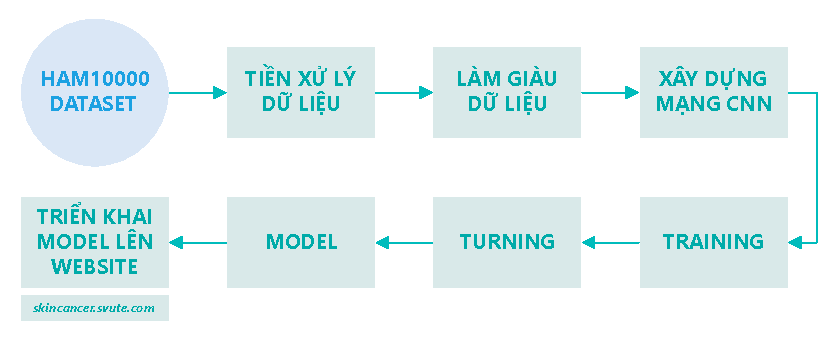
\includegraphics[width=\linewidth]{./images/quatrinh.eps}
		\caption{Phân bố dữ liệu tập HAM10000.}
		\label{fig:quatrinh}
	\end{figure}
	
	\subsection{Tập dữ liệu HAM10000}
	
	HAM10000 là tập dữ liệu được sử dụng trong đề tài này là bộ dữ liệu được công khai bởi đại học Hardvard. Bộ dữ liệu bao gồm 10015 ảnh soi da để phục vụ tạo ra một tiêu chuẩn trong việc chẩn đoán các bệnh về tổn thương da.Tập dữ liệu HAM10000 được sử dụng trong cuộc thi ISIC 2018, trong tập dữ liệu có 7 lớp và 7 lớp này là 7 loại bệnh về tổn thương da cụ thể ở bảng dưới đây.
	
	\begin{center}
		\begin{tabular}{|l|c|}
			\hline
			\rowcolor[HTML]{333333} 
			\multicolumn{1}{|c|}{\cellcolor[HTML]{333333}{\color[HTML]{FFFFFF} \textbf{Loại bệnh}}} & {\color[HTML]{FFFFFF} \textbf{Nhãn}} \\ \hline
			Actinic keratoses                                                                       & 0                                    \\ \hline
			Basal cell carcinoma                                                                    & 1                                    \\ \hline
			Benign keratosis-like lesions                                                           & 2                                    \\ \hline
			Dermatofibroma                                                                          & 3                                    \\ \hline
			Malignant Melanoma                                                                      & 4                                    \\ \hline
			Melanocytic nevi                                                                        & 5                                    \\ \hline
			Vascular lesions                                                                        & 6                                    \\ \hline
		\end{tabular}
	\captionof{table}{Phân lớp các loại bệnh trong tập dữ liệu HAM10000}
	\end{center}

	\noindent
	Tập dữ liệu HAM10000 bị vấn đề về mất cân bằng dữ liệu như hình dưới đây, trong tập dữ liệu này số lượng ảnh về bệnh "Melanocytic nevi" chiếm số lương rất lớn\\	
	
	
	\begin{figure}[h!]
		\centering
		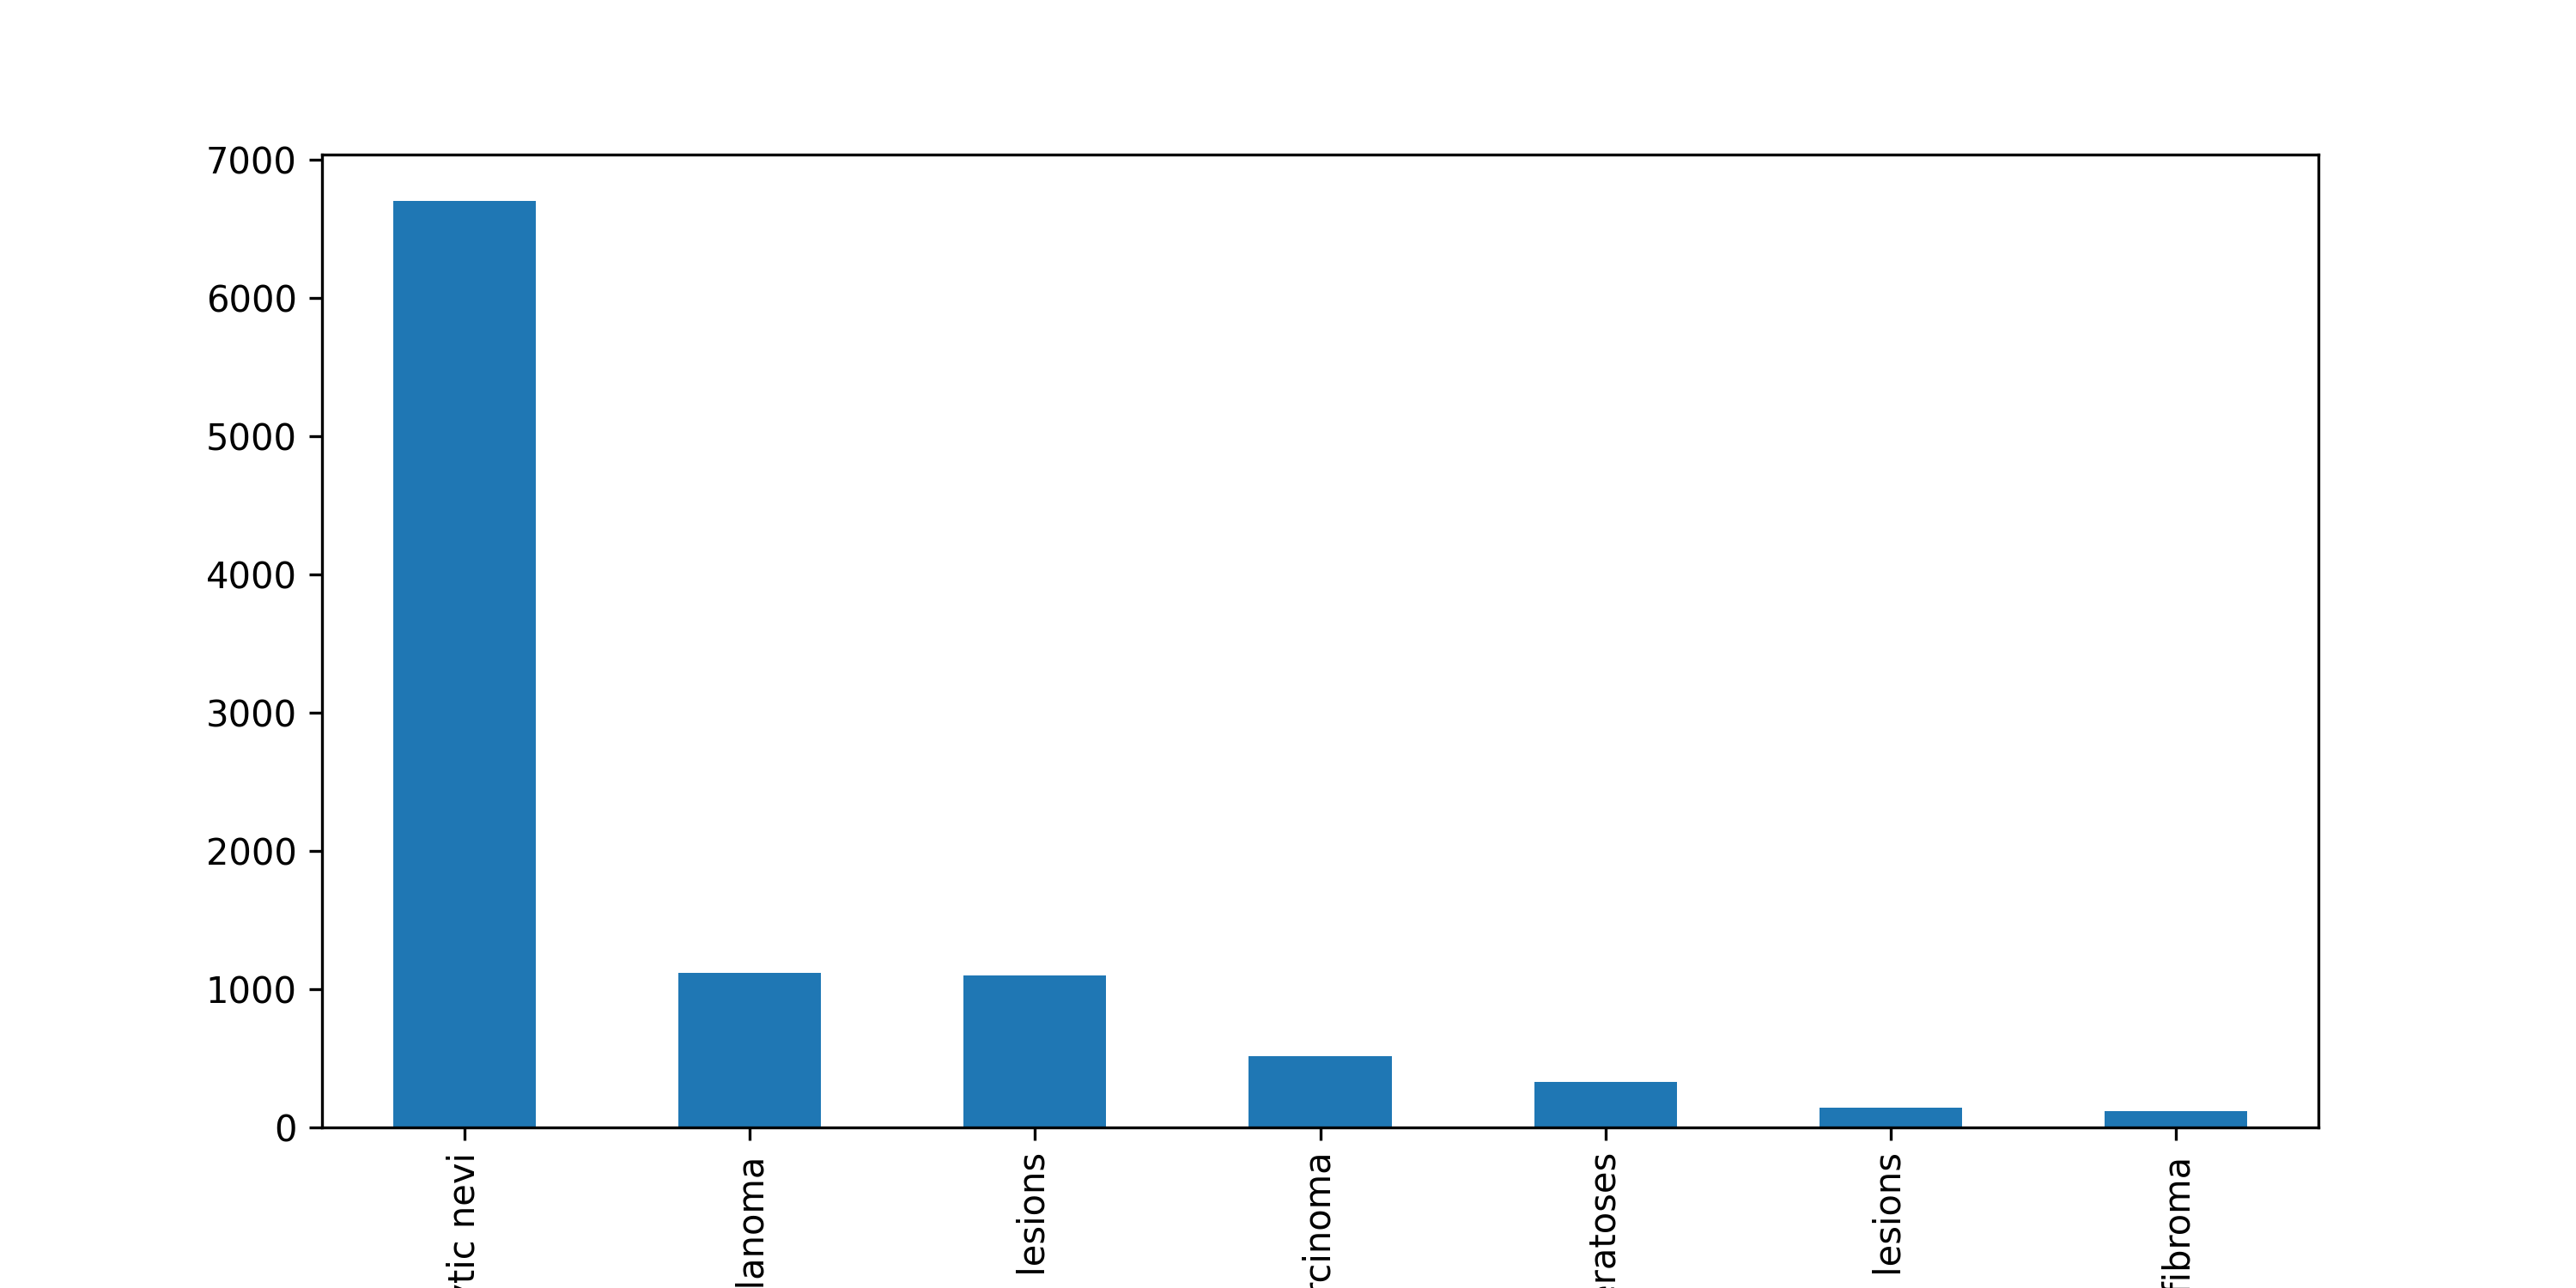
\includegraphics[width=0.5\linewidth]{./images/imbalance.png}
		\caption{Phân bố dữ liệu tập HAM10000.}
		\label{fig:ham10000}
	\end{figure}

	\begin{center}
		\begin{tabular}{|l|c|c|c|c|c|c|c|l|}
			\hline
			\rowcolor[HTML]{000000} 
			{\color[HTML]{FFFFFF} \textbf{Phân lớp}} & {\color[HTML]{FFFFFF} \textbf{0}} & {\color[HTML]{FFFFFF} \textbf{1}} & {\color[HTML]{FFFFFF} \textbf{2}} & {\color[HTML]{FFFFFF} \textbf{3}} & {\color[HTML]{FFFFFF} \textbf{4}} & {\color[HTML]{FFFFFF} \textbf{5}} & {\color[HTML]{FFFFFF} \textbf{6}} & {\color[HTML]{FFFFFF} \textbf{Tổng}} \\ \hline
			\textbf{Số lượng hình ảnh}               & 327                               & 514                               & 1099                              & 115                               & 6705                              & 142                               & 1113                              & 10015                                \\ \hline
		\end{tabular}
	\captionof{table}{Số lượng ảnh trong tập dữ liệu HAM10000}
	\end{center}
	
	
	
	\subsection{Tiền xử lý dữ liệu}
	
	\subsection{Cấu trúc mạng CNN}
	
	\subsection{Công cụ đánh giá mô hình}
	
	%%%%%%%%%%%%%%%%%%%%%%%%%%%%%%%%%%%%%%%%%%%%%%%
	
	\section{Kết quả}
	
	%%%%%%%%%%%%%%%%%%%%%%%%%%%%%%%%%%%%%%%%%%%%%%%
	
	\section{Kết luận}
\end{document}